\section{Learning by mimesis model}
\label{cha5:sec2}

We adopt the mimesis model to learn motion primitives of manipulation from human demonstrations. In this approach, the demonstrated motions are firstly encoded by the Hidden Markov Model (HMM)~\citep{rabiner1989tutorial}. A topological space, i.e. proto symbol space, is then constructed to represent the similarities between the HMMs. In this space, each HMM is abstracted to a labelled point: the proto symbol. New motions are generated as new proto symbols. The correlation between the location of the new proto symbols and their physical effects is learnt by regression. This correlation allows us to directly query a new motion from a high level task requirement.

In short, the general approach has 5 steps as listed underneath:

\begin{enumerate}
\item {\bf{Human demonstration of motion primitives}}: A human teacher demonstrates manipulation motion primitives (Section~\ref{cha5:sec2:demonstration}).
\item {\bf{Motion symbolization}}: Abstract the motion primitives by HMM and create the proto-symbol space (Section~\ref{cha5:sec2:symbolization}).
\item {\bf{Motion interpolation}}: Interpolate the proto-symbol space and construct new HMM.  (Section~\ref{cha5:sec2:interpolation}).
\item {\bf{New motion generation}}: Generate motion using proto-symbols (Section~\ref{cha5:sec2:generating}).
\item {\bf{Learning motion effects}}: Robot reproduces the motion and learns the correlation between the location of the proto-symbols and the effect of the generated motions (Section~\ref{cha5:sec2:learning}).
%\item {\bf{Generating}}: Given a unseen object, choose a proper point in the proto-symbol space and generate the corresponding motion sequence to grasp the object (Section 3E).
\end{enumerate}



\subsection{Human demonstration of motion primitives}
\label{cha5:sec2:demonstration}
%To design a adaptive motion primitive, demonstrations showing different scenarios are required.
The motion primitives of manipulation are first demonstrated by a human. The same primitives were demonstrated a few times so that the HMM is able to encode the general features of the movement. Each primitive has its own purpose and distinct pattern. To enable the robot to work in different task contexts, different primitives need to be demonstrated. For example, to design a motion primitive for fetching boxes in different sizes (size is the task context), we need to demonstrate at least two primitives: grasping a small box and grasping a big box (Figure.~\ref{fig:bimanual}). Grasping a box with the size between the big one and the small one is achieved by interpolation between these primitives. For more complex motion, more than two primitives may be required to achieve the desired motions.

%Later in the interpolation step (section~\ref{sbsec:interpolation}), new motions are generated by combining the demonstrated motions.
In this approach, the demonstrated motions do not only provide the dynamics of the motion primitives, but also define the feasibilities of the motion primitives. In the example given above of grasping different sizes of boxes, one should demonstrate the motion primitive for grasping the smallest feasible box and the other for grasping the biggest feasible box. Here the ``feasibility'' is defined according to the limitation of the robot joints. As the new motions are interpolations of the demonstrations, joint limits or singularities can be avoided in the new motions by well chosen demonstrations.

\begin{figure}
\centering
  \subfloat[ {}]{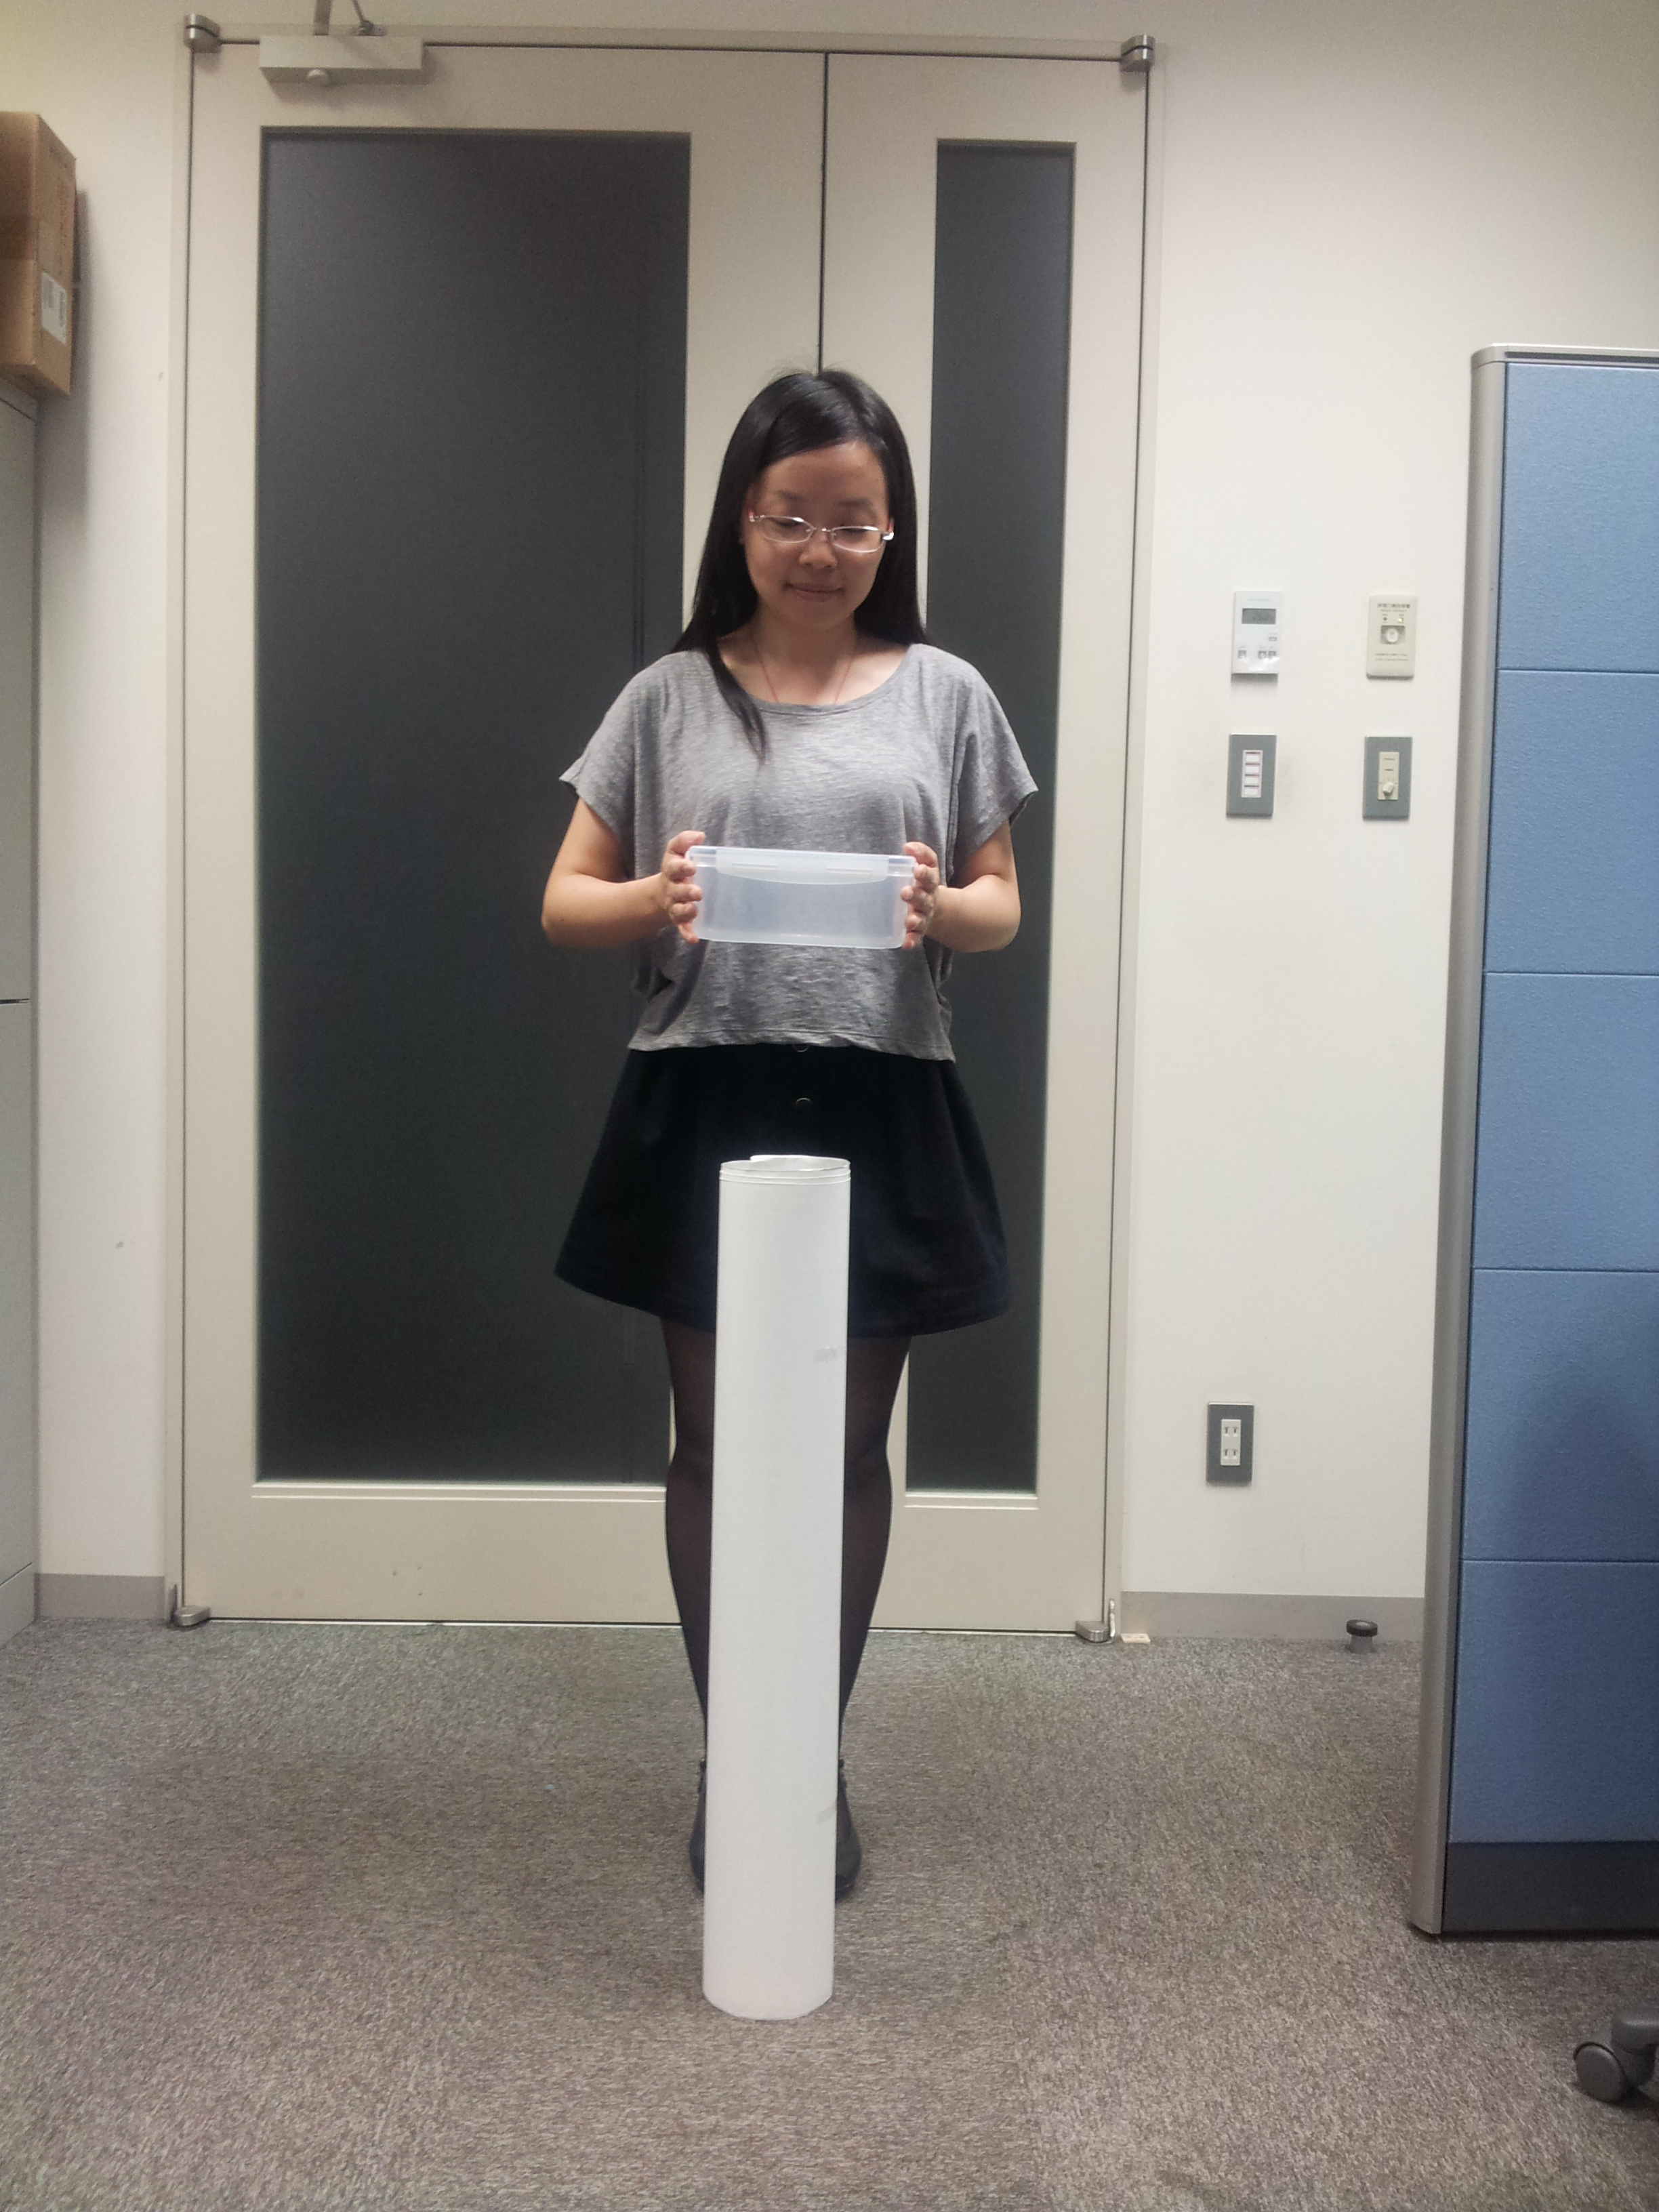
\includegraphics[width=5cm]{./fig_cha5/gsbox.jpg}}
  \subfloat[ {}]{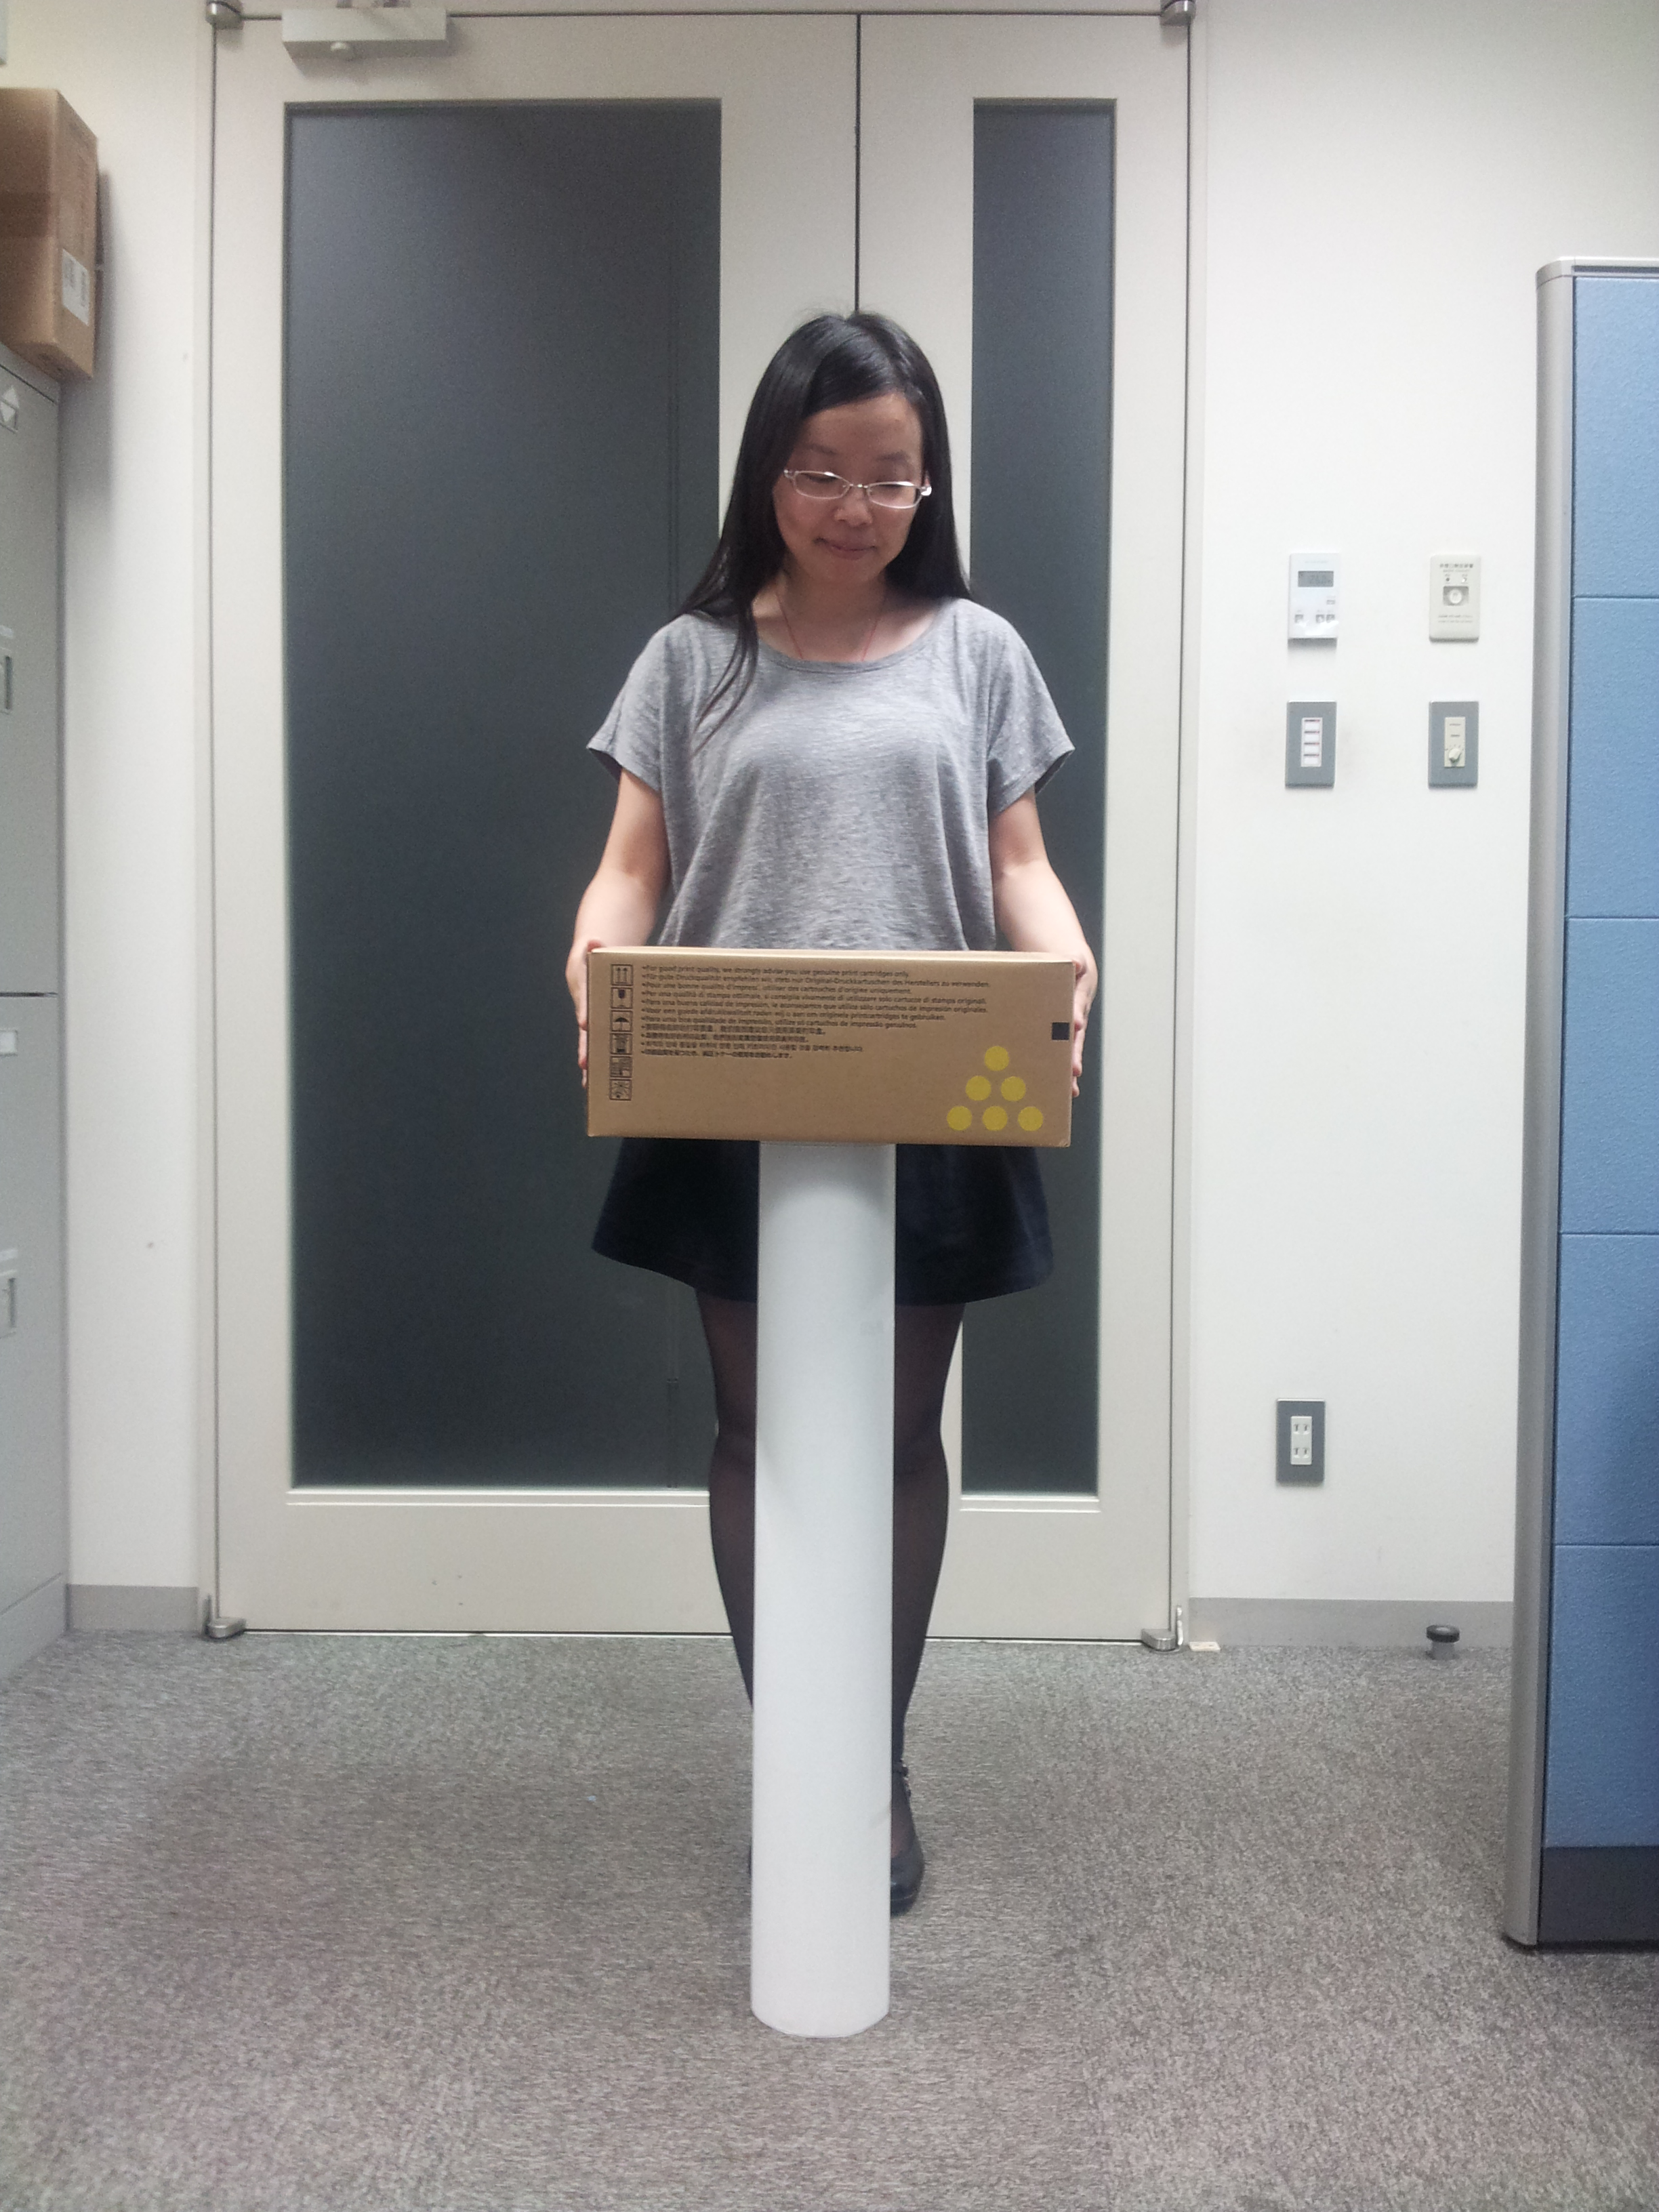
\includegraphics[width=5cm]{./fig_cha5/gpinkbox.jpg}}
  \caption{  {Human bimanual grasps. (a) Human grasping a small box. (b) Human grasping a big box.}}
  \label{fig:bimanual}
\end{figure}


\subsection{Motion symbolization}
\label{cha5:sec2:symbolization}
%The demonstrated motion sequences are then adapted to a 20 degrees of freedom humanoid, the HOAP robot~\citep{inamura2004embodied}.
In order to store and label the observed motions, we construct the ``proto-symbol space''. This is done in two steps: first encode the motion patterns as HMM's, and second project them to be a set of ``proto-symbols'' in the proto-symbol space, where the similarity between different motion patterns are represented by the Euclidean distance.

\paragraph{Hidden Markov Model} ~\\
%TODO: more HMM
%TODO: more forward-backward procedure
A Hidden Markov Model is a stochastic mathematical model for sequential data. It describes a data sequence as a Markov process, with which the data is described by transitions between a set of states. In a Markov process, the future state of the process depends solely on its current state. It can be thought of as a 'memory-less' process: it only need to 'remember' the current state but not the whole process' history, in order to predict the future. This is a strong assumption.
Temporal patterns with this characteristic, e.g. speech, handwriting and sequences of body movements, can be approximated by a Markov model. In a simple Markov process, the transitions between states are directly visible. Conversely, the states of hidden Markov Model is not directly visible, i.e. hidden.

An HMM has two layers: the hidden states and the outputs. The outputs are directly visible but their pattern is controlled by the hidden states. The way the hidden states transit to each other and the way they emit to the outputs determine the output pattern. Though they are not directly visible, the hidden states can be inferred by the observable outputs. A well known application of HMM is speech recognition. Speech recognition systems use HMM to analyze the signal of speech in order to discover the meaning. Here the sound of the speech is the observable output and the meaning of the speech is the hidden state.


A HMM can be fully described by a triple $\left(\pi,\boldsymbol{A},\boldsymbol{B}\right)$:

\begin{enumerate}
\item $\pi$: the vector of the initial probabilities of each state.
\item $\boldsymbol{A}={a_{ij}}$: the state transition matrix. This is the probability that one state ($q_i$) transits to another ($q_j$): $Pr\left(q_i{\mid}q_j\right)$.
\item $\boldsymbol{B}={b_{ij}}$: the output probability (confusion matrix). This is the probability that one state ($q_j$) produces an output ($o_i$): $Pr\left(o_i{\mid}q_{j}\right)$. If the outputs are discrete, i.e. have a countable number of states, this can be simply represented by a matrix. If the outputs are continuous, the output probability is usually described by a GMM.
\end{enumerate}

Figure~\ref{fig:chmm} illustrates the mechanism of a HMM encoding a motion pattern. This is a left-to-right Continuous Hidden Markov Model (CHMM). In a general HMM, the hidden states can transition to any other states. In a left-to-right HMM the transition has more constraints. The states are placed in a ``left to right'' order, each state can only transition to the state at its right or transition to back to itself, the possibility of it transiting to any other states is zero. A left-to-right HMM restricts the complexity of the data pattern it can model and is adequate for modelling motion primitives.

To encode the motion primitives by HMM, we define the pattern by: $\lambda$ = $\{\boldsymbol{Q},\pi,\boldsymbol{A},\boldsymbol{B}\}$, where $\boldsymbol{Q}=\{q_1, ..., q_N\}$ is a finite set of states, $\pi$ is the the initial distribution, $\boldsymbol{A}=\{a_{ij}\}$ is the state transition probability matrix denoting the probability that node $q_i$ transits to $q_j$ and $\boldsymbol{B}=\{b_{i}\}$ is the continuous output probabilities denoting the probability distribution that the output vector $o[t]$ is given by $q_i$. The $\pi$ is the same as for each CHMM as we use a left-to-right CHMM model. Therefore, the parameter set $\mathcal{P} = \{a_{ij},b_i\}$ characterizes the behaviour of the motion primitive. We call $\mathcal{P}$ a proto-symbol.

The CHMM is learned using the Baum-Welch algorithm~\citep{rabiner1989tutorial}\footnote{We use the Hidden Markov Model Toolkit (HTK) to learn the HMM}.
For simplicity, we use a single Gaussian model for the output of each node in the CHMM. This allows us to synthesise new motion simply by interpolating the means and covariances of the Gaussians (Section~\ref{cha5:sec2:interpolation}).

The proto-symbol space is constructed to represent the similarity between CHMMs. This requires us to compute the similarity between each pair of CHMMs. In this work, we use the Bhattacharyya distance~\citep{kailath1967divergence} as our similarity metric, as it is a symmetric metric with respect to two probability variables. The Bhattacharyya distance $BD(p,q)$ between two Gaussian distributions $p(x;\mu_p,\Sigma_p)$ and $q(x;\mu_q,\Sigma_q)$ is defined as follows:


\begin{figure}[t!]
  \centering
  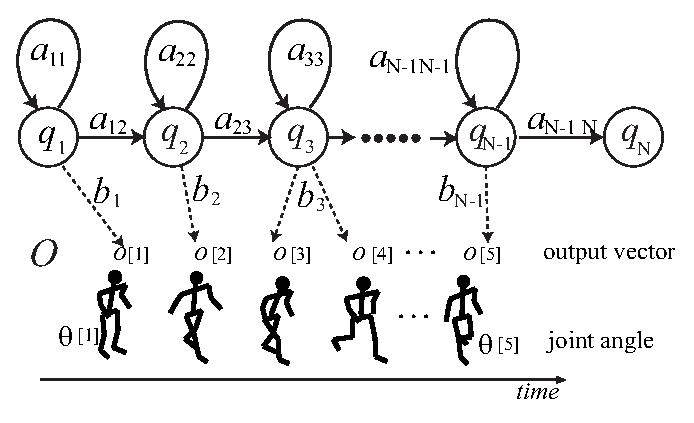
\includegraphics[width=12cm]{./fig_cha5/chmm.eps}
  \caption{{An illustration of encoding a motion by Continuous Hidden Markov Model\protect\footnotemark.}
}
    \label{fig:chmm}
\end{figure}

\footnotetext{Reprinted with permission.}

%\begin{equation}
\begin{align}
\begin{split}
&BD(p,q) = -log\int^{\infty}_{-\infty}\sqrt{p(x)q(x)}dx \\
=\frac{1}{8}&\mu_{pq}\left({\frac{\Sigma_p+\Sigma_q}{2}}\right)^{-1}\mu_{pq}^T +\frac{1}{2}log{\frac{\mid\frac{\Sigma_p+\Sigma_q}{2}\mid}{\mid\Sigma_p\mid^{\frac{1}{2}}\mid \Sigma_q\mid^{\frac{1}{2}}}}
\end{split}
\end{align}
%\end{equation}
where
\begin{equation}
\mu_{pq} = \mu_p - \mu_q
\end{equation}

The Bhattacharyya distance DB($\lambda_1, \lambda_2$) between two HMMs is computed by summing the distances between the Gaussian distributions, i.e. the output probability distributions for the nodes:

\begin{align}
\begin{split}
&DB(\lambda_1, \lambda_2) = \\
&\sum_i\sqrt{BD\left(\mathcal{N}_{1i}\left(\mu_{1i},\Sigma_{1i}\right), \mathcal{N}_{2i}\left(\mu_{2i},\Sigma_{2i}\right)\right)}
\end{split}
\end{align}
where $\mathcal{N}_{ji}(\mu_{ji},\Sigma_{ji})$ is the output probability at the $i$-th node $q_i$ of the HMM $\lambda_i$.

The proto-symbol space is constructed by the multi-dimensional scaling technique (MDS)~\citep{schiffman1981introduction}. This technique computes the locations of the CHMMs in the proto-symbol space by minimizing the criterion:

\begin{equation}
S^2 = \sum_{i,j}\left(DB_{ij}-d_{ij}\right)
\end{equation}
where $DB_{ij}$ is the Bhattacharyya distance between the $i$th and $j$th CHMMs and $d_{ij}$ is their Euclidean distance between their proto-symbols. %Figure~\ref{pss} shows an proto-symbol space constructed by 4 proto-symbols.



\subsection{Motion interpolation}
\label{cha5:sec2:interpolation}
To generate new motions, new locations in the proto-symbol space are explored. This is done by interpolation between different proto-symbols.
%For the same set of motion primitives, the number of states are the same and hence the motions can be mixed in the time domain.
In the left-to-right model, the expected duration $s_i$ of the state $q_i$ can be computed as

\begin{equation}
\label{sequation}
s_i = \sum_{n=1}^{\infty} n(1-a_{ii})a_{ii}^{n-1} = \frac{1}{1-a_{ii}},
\end{equation}
where $a_{ii}$ is the probability of self-transition at the state $q_i$.

A new proto-symbol $\hat{\mathcal{P}}$ is expressed by the linear combination of $m$ proto-symbols $(\mathcal{P}_1, ..., \mathcal{P}_m)$. The weights of different proto-symbols are expressed by the mix coefficient $c_j$. The expected duration $\hat{s}_i$ for the new motion in the state $q_i$ is computed as

\begin{equation}
\hat{s}_i = \sum_j^mc_js_i^{(j)}
\label{s}
\end{equation}
with this we can compute the new state transition probability $\hat{a}_{ii}$ as

\begin{equation}
\hat{a}_{ii} = \frac{\hat{s}_i-1}{\hat{s}_i}
\end{equation}
Note that according to the Eq.~\ref{s}, $s_i\ge1$ and hence the following constraint must be satisfied

\begin{equation}
\sum_j^m\frac{c_j}{1-a^j_{ii}} \ge 1
\end{equation}

To compute the new output probability $b_i$, since there is only one Gaussian in each state, we simply sum the means and variances of the Gaussians of the same state as

\begin{equation}
\hat{b}_i(O) = \mathcal{N}(O;\hat{\boldsymbol{\mu}}_i,\hat{\boldsymbol{\sigma}}_i^2) = \sum_j^m{c_jb_i^{(j)}(O)}
\end{equation}
where
\begin{equation}
\hat{\boldsymbol{\mu}}_i = \sum_j^mc_j\boldsymbol{\mu}_i^{(j)}
\end{equation}

\begin{equation}
\hat{\boldsymbol{\sigma}}_i^2 = \sum_j^mc_j^2{\boldsymbol{\sigma}_i^{(j)}}^2
\end{equation}
$\mu_i^{(j)}$ and ${\sigma_i^{(j)}}$ are the mean and variance of the Gaussian representing the $i$-th state.

In theory this method can also be used to extrapolate the proto-symbols with negative mixing coefficients, which allows us to explore outside the feasible region defined by the demonstrations. This can generate motions that are beyond our experience however the feasibility cannot be guaranteed, i.e. this may gives joint angles over the robot's limit.

\subsection{Motion generation}
\label{cha5:sec2:generating}
A new motion sequence is generated from the new proto-symbols by using an averaging method~\citep{inamura2004embodied}.
%The basic idea is to decode a motion sequence from the CHMMs by averaging over repetition of motion generation.
The steps of generation are as follows :

\begin{enumerate}
\item: Starting from a node $q_1$, let the motion element sequence be $O = \phi$.
\item: Use the transition probability $\{a_{ij}\}$ to generate the states $q_j$.
\item: Use the output probabilities $\{b_i\}$ to decide the output label $o_k$.
\item: Add the output label $o_k$ to the motion elements sequence $O$.
\item: Stop when the generation process reaches the end node $q_N$.
\end{enumerate}

Due to the stochastic nature of this method, motions generated by the same HMM are not identical at each time. Nevertheless, they have the same dynamics as they are generated from the same parameters $\boldsymbol{A}$ and $\boldsymbol{B}$. We repeat the above steps and average the generated motions to produce the final motion. As the duration of each generated motion is different, prior to averaging we match the time in each motion by:

\begin{equation}
\bar{\theta}\left(t\right)=\theta\left(T\frac{t}{T_{adv}}\right)
\end{equation}

where $T$ is the time duration of each motion, and $T_{adv}$ is the average time duration of all motions. This step normalize all motions in the scale of time.

\subsection{Learning motion effects}
\label{cha5:sec2:learning}

In contrast to free body motions, the motion of object manipulation needs to achieve certain outcomes, such as grasping a given size of box. However the physical effects of the demonstrated and generated motions are unknown, as the robot has a different embodiment to the human demonstrator. For example, the motion for a human to grasp a 30$cm$ length box may only allow the robot to grasp a 15$cm$ length box. Therefore, a learning process is needed to quantify the correlation between the location of the new proto-symbol and its physical effect.

To do this, we first interpolate the proto-symbol space with a few different mixing coefficients. We then generate the corresponding motions and perform them with a robot. The platform we used is the iCub in the Webots simulator. As the iCub has the same joint configuration of arm as the one provided by Kinect, we directly apply the generated motions to the iCub.  The outcome of the motion, for example the size of the box the robot can grasp with the motion, are recorded with their corresponding mixing coefficients.

The correlation between the sizes and the mixing coefficients is then found by regression analysis. Figure~\ref{regression} shows an example of the result of the regression. With this result, we are able to infer the mixing coefficient for generating a proper motion. By using the method detailed in section~\ref{cha5:sec2:generating}, the motion with a desired effect can be generated. Our experiments verify that this method can generate new grasping motions and the result will be discussed in the next section in detail. 